\documentclass[12pt, a4paper]{article}

% ==========================================
% 1. KHAI BÁO GÓI THƯ VIỆN (PACKAGES)
% ==========================================
% Bảng mã & Font chữ
\usepackage[utf8]{inputenc}
\usepackage[T5]{fontenc}

% Toán học
\usepackage{amsmath, amssymb}

% Căn lề & Bố cục trang
\usepackage[top=2.2cm, bottom=1.5cm, left=1cm, right=1cm, headheight=15pt]{geometry}
\usepackage{fancyhdr}
\usepackage{needspace}
\usepackage{tkz-tab}

% Đồ họa & Màu sắc
\usepackage{xcolor}
\usepackage{graphicx} 
\usepackage{tikz}
\usetikzlibrary{calc, shapes.geometric, positioning}


% Bảng biểu & Danh sách
\usepackage{colortbl}
\usepackage{array}
\usepackage{makecell}
\usepackage{multirow}
\usepackage{tasks}

% Biểu tượng
\usepackage{fontawesome5}

% ==========================================
% 2. THIẾT LẬP MÀU SẮC CHỦ ĐẠO
% ==========================================
\definecolor{goldyellow}{RGB}{255, 179, 0}
\definecolor{amberorange}{RGB}{230, 115, 0}
\definecolor{lightamber}{RGB}{255, 248, 225}
\definecolor{deepblue}{RGB}{25, 42, 86}
\definecolor{accentred}{RGB}{232, 65, 24}
\definecolor{softgray}{RGB}{220, 220, 222} 
\definecolor{fbblue}{RGB}{15, 80, 200}


% ==========================================
% 3. CẤU HÌNH HEADER & FOOTER
% ==========================================
\pagestyle{fancy}
\fancyhf{}
\renewcommand{\headrulewidth}{0pt}

% Khai báo biến lưu trữ nội dung góc phải của Header
\newcommand{\HeaderRightText}{}

% --- Header ---
\fancyhead[C]{
    \begin{tikzpicture}[remember picture, overlay]
        
        % Dải màu trang trí góc trên
        \path[fill=deepblue] (current page.north west) -- (current page.north east) 
            -- ($(current page.north east) + (0, -1.6cm)$) 
            .. controls ($(current page.north) + (3, -2.0cm)$) and ($(current page.north) + (-3, -0.4cm)$) .. 
            ($(current page.north west) + (0, -1.0cm)$) -- cycle;
            
        \path[fill=goldyellow] (current page.north west) -- (current page.north east) 
            -- ($(current page.north east) + (0, -1.0cm)$) 
            .. controls ($(current page.north) + (4, -1.0cm)$) and ($(current page.north) + (-2, -2.2cm)$) .. 
            ($(current page.north west) + (0, -1.6cm)$) -- cycle;
            
        \path[fill=amberorange] (current page.north west) -- ($(current page.north west) + (6.5cm, 0)$) 
            .. controls ($(current page.north west) + (4.5cm, -1.2cm)$) and ($(current page.north west) + (2cm, -2.0cm)$) .. 
            ($(current page.north west) + (0, -2.0cm)$) -- cycle;
            
        % Logo góc trái Header
        \node[anchor=west, inner sep=0pt] 
            at ($(current page.north west) + (0cm, -0.8cm)$) {
\includegraphics[height=2.0cm]{../../../image/logo-header.png}};
            
        % Text góc phải Header (Tự động lấy từ đối số thứ 3 của \titlebox)
        \node[anchor=east, text=white, font=\small\bfseries\sffamily] 
            at ($(current page.north east) + (-0.8cm, -0.5cm)$) {\HeaderRightText};
    \end{tikzpicture}
}

% --- Footer ---
\fancyfoot[C]{
    \begin{tikzpicture}[remember picture, overlay]
        % Đường kẻ ngang
        \draw[amberorange, line width=1.5pt] 
            ($(current page.south west) + (0cm, 0.4cm)$) -- ($(current page.south east) + (0cm, 0.4cm)$);

        % Dải cong góc phải
        \path[fill=goldyellow] (current page.south east) -- ($(current page.south east) + (-5cm, 0)$) 
            .. controls ($(current page.south east) + (-3cm, 0.8cm)$) and ($(current page.south east) + (-1.5cm, 1.2cm)$) .. 
            ($(current page.south east) + (0, 1.2cm)$) -- cycle;

        % Mạng xã hội
        \node[anchor=west, inner sep=0pt] at ($(current page.south west) + (1cm, 0.8cm)$) {
            \small\sffamily
            \textcolor{fbblue}{\faFacebook\hskip 4pt Toán Anh Huy MATH-STER}
            \hskip 18pt
            \textcolor{black}{\faTiktok\hskip 4pt huymathster}
        };

        % Số trang
        \node[circle, fill=white, draw=amberorange, line width=1.5pt, text=deepblue, font=\large\bfseries\sffamily, inner sep=4pt, minimum size=0.8cm] 
            at ($(current page.south east) + (-1.2cm, 0.6cm)$) {\thepage};
    \end{tikzpicture}
}

% ==========================================
% 4. ĐỊNH NGHĨA MACRO: KHUNG TIÊU ĐỀ
% ==========================================
\newcommand{\titlebox}[3]{
    % Gán nội dung đối số #3 vào biến HeaderRightText
    \gdef\HeaderRightText{#3}
    
    \begin{center}
    \vspace*{-0.5cm}
    \begin{tikzpicture}
        % Khung vô hình (Phantom Box) định chuẩn kích thước
        \node[text width=16cm, inner xsep=0pt, inner ysep=16pt, opacity=0] (MainBox) {
            \begin{minipage}[c]{4.2cm}
                \centering\vspace{0.1cm}
                \rule{2.2cm}{2.2cm} 
                \vspace{0.1cm}
            \end{minipage}%
            \begin{minipage}[c]{11.5cm}
                \centering\vspace{0.15cm}
                {\huge\bfseries\sffamily #2 \par}
                \vspace{0.15cm} 
            \end{minipage}
        };
        
        % Đổ bóng & Nền
        \fill[goldyellow, rounded corners=8pt] ([xshift=5pt, yshift=-5pt]MainBox.south west) rectangle ([xshift=5pt, yshift=-5pt]MainBox.north east);
        \fill[white, rounded corners=8pt] (MainBox.south west) rectangle (MainBox.north east);
        
        % Lưới ô ly & Nền Logo
        \begin{scope}
            \clip[rounded corners=8pt] (MainBox.south west) rectangle (MainBox.north east);
            \draw[step=0.4cm, softgray!50, line width=0.6pt] (MainBox.south west) grid (MainBox.north east);
            \fill[lightamber!60] (MainBox.south west) rectangle ([xshift=4.2cm]MainBox.north west);
        \end{scope}

        % Viền ngoài
        \draw[deepblue, line width=1.5pt, rounded corners=8pt] (MainBox.south west) rectangle (MainBox.north east);

        % Nội dung Text (Lớp trên cùng)
        \node[text width=16cm, inner xsep=0pt, inner ysep=16pt] at (MainBox.center) {
            \begin{minipage}[c]{4.2cm}
                \centering
                % --- ĐIỀU CHỈNH TỌA ĐỘ LOGO Ở ĐÂY ---
                \hspace*{-0.5cm}\raisebox{-0.2cm}{
\includegraphics[width=5.5cm]{../../../image/logo.png}}
            \end{minipage}%
            \begin{minipage}[c]{11.5cm}
                \centering\vspace{0.15cm}
                {\huge\bfseries\sffamily\color{deepblue} #2 \par}
                \vspace{0.15cm} 
            \end{minipage}
        };
        
        % Trang trí phụ kiện
        \draw[deepblue, line width=1.5pt, dashed] ([xshift=4.2cm]MainBox.north west) -- ([xshift=4.2cm]MainBox.south west);
        \node[regular polygon, regular polygon sides=4, rotate=45, fill=white, draw=accentred, line width=1.2pt, inner sep=2.5pt] at ([xshift=4.2cm]MainBox.west) {};
        \node[anchor=west, fill=amberorange, text=white, font=\large\bfseries\sffamily, rounded corners=4pt, draw=deepblue, line width=1.5pt, inner xsep=12pt, inner ysep=6pt] at ([xshift=1.5cm]MainBox.north west) {#1};
        \fill[accentred] ([xshift=-1.8cm, yshift=-0.4cm]MainBox.north east) circle (3pt);
        \fill[amberorange] ([xshift=-1.4cm, yshift=-0.4cm]MainBox.north east) circle (3pt);
        \fill[goldyellow] ([xshift=-1.0cm, yshift=-0.4cm]MainBox.north east) circle (3pt);
    \end{tikzpicture}
    \vspace*{0cm}
    \end{center}
}

% ==========================================
% 5. ĐỊNH NGHĨA MACRO: CẤU TRÚC CÂU HỎI (ÉP SÁT NHAU)
% ==========================================
\newcommand{\questioncore}[2]{
    % Xóa khoảng cách phía trên, ép sát câu trước
    \noindent \textbf{\textcolor{deepblue}{Câu #1.} \textcolor{accentred}{[STER]}} #2
    \par\nopagebreak
}

% Cấu hình hiển thị đáp án trắc nghiệm
\settasks{
    label=\textbf{\textcolor{amberorange}{\Alph*.}}, 
    label-width=15pt,     
    item-indent=25pt,     
    label-offset=6pt,    
    column-sep=20pt,     
    after-item-skip=2pt  % Đã giảm tối đa khoảng cách giữa các dòng đáp án A B C D
}

% Hàm vẽ dòng kẻ nháp
\newcommand{\drawdashlines}[1]{
    \ifnum#1>0
        \nopagebreak\vspace{0.1cm}\noindent 
        \begin{tikzpicture}
            \foreach \i in {1,...,#1} {
                \draw[softgray, line width=0.2pt] (0,-{\i}) -- (\textwidth-4pt,-{\i});
            }
        \end{tikzpicture}
        \par
    \fi
    % Đã xóa hoàn toàn khoảng cách thừa ở nhánh else
}

% --- Dạng 1: Trắc nghiệm 4 đáp án ---
\newcommand{\questionLinesManual}[4]{
    \pgfmathsetmacro{\calculatedSpace}{1.5 + #1 * 0.65}
    \needspace{\calculatedSpace cm} 
    \questioncore{#2}{#3}
    #4
    \par\nopagebreak
    \drawdashlines{#1}
}


% --- Dạng 2: Trắc nghiệm Đúng/Sai ---
\newcommand{\questionTrueFalse}[4]{
    \scriptsize
    \pgfmathsetmacro{\calculatedSpace}{3.0 + #1 * 0.65} 
    \needspace{\calculatedSpace cm}
    \questioncore{{#2}}{#3}
    
    \nopagebreak
    \begin{flushleft}
    \renewcommand{\arraystretch}{1.2} % Bóp nhỏ chiều cao của bảng Đ/S
    \begin{tabular}{|>{\centering\arraybackslash}m{0.4cm}|m{6cm}|>{\centering\arraybackslash}m{1cm}|>{\centering\arraybackslash}m{1cm}|}
        \hline
        \rowcolor{amberorange!20}
        & \multicolumn{1}{>{\centering\arraybackslash}m{6cm}|}{\textbf{\textcolor{deepblue}{Mệnh đề}}} & 
        \textbf{\textcolor{deepblue}{Đúng}} & 
        \textbf{\textcolor{deepblue}{Sai}} \\
        \hline
        #4
        \hline
    \end{tabular}
    \renewcommand{\arraystretch}{1}
    \end{flushleft}
    
    \par\nopagebreak
    \drawdashlines{#1}
}

% ----- Dạng 3: Tự luận ngắn -----
\newcommand{\questionShortAnswer}[3]{
    \scriptsize
    \pgfmathsetmacro{\calculatedSpace}{1.5 + #1 * 0.8}
    \needspace{\calculatedSpace cm}
    
    {\linespread{1.1}\selectfont % Bóp nhỏ giãn dòng của câu tự luận
    \questioncore{#2}{#3}\par}
    
    \nopagebreak
    \begin{flushright}
        \begin{tikzpicture}
            \node[anchor=east, font=\small\bfseries\sffamily, text=deepblue] 
                at (-0.2, 0.4) {Đáp án:};
            \fill[goldyellow, rounded corners=3pt] (0.08, -0.08) rectangle (3.08, 0.72);
            \draw[draw=deepblue, fill=white, line width=1.2pt, rounded corners=3pt] 
                (0,0) rectangle (3.0, 0.8);
            \foreach \x in {0.75, 1.5, 2.25} {
                \draw[draw=deepblue, line width=0.6pt] (\x, 0) -- (\x, 0.8);
            }
        \end{tikzpicture}
    \end{flushright}
    
    \par\nopagebreak
    \drawdashlines{#1}
}

% ==========================================
% BẮT ĐẦU NỘI DUNG TÀI LIỆU
% ==========================================
\begin{document}

% Truyền 3 tham số: {Nhãn cam} {Chữ to chính giữa} {Chữ ở góc phải Header}
\titlebox{Chủ đề: Hàm số}{Ứng dụng khảo sát đồ thị hàm số}{Hàm số: Ứng dụng đồ thị}


\questionTrueFalse{12}{1}{Chủ một quán cà phê ghi nhận số lượng khách trung bình của mỗi ngày sau \( t \) tuần khai trương (từ tuần thứ nhất đến tuần thứ 40). Bằng cách kiểm đếm và thống kê số lượng đơn hàng, người đó đã thống kê được số liệu như sau:

\begin{table}[h!]
\centering
\renewcommand{\arraystretch}{1.8} % Tăng khoảng cách dòng để chữ không bị dính vào đường kẻ
\begin{tabular}{|c|c|c|c|c|}
\hline
$t$ (tuần) & 4 & 6 & 8 & 12 \\ \hline
\begin{tabular}[c]{@{}c@{}}Số khách trung\\ bình mỗi ngày\end{tabular} & 100 & 130 & 150 & 175 \\ \hline
\end{tabular}
\end{table}

Biết rằng hàm mô tả số lượng khách trung bình mỗi ngày có dạng \( y = \dfrac{at + b}{ct + d} \) (\( ad - bc \neq 0, c \neq 0 \)).}{
    \textbf{a)} & Hàm số mô tả số lượng khách trung bình mỗi ngày của quán cà phê là \( y = \dfrac{250t + 200}{t + 4} \).
    & \textcolor{amberorange}{$\bigcirc$} & \textcolor{amberorange}{$\bigcirc$} \\ \hline
    
    \textbf{b)} & Tại thời điểm sau tuần thứ 11, số lượng khách hàng trung bình mỗi ngày của quán cà phê là 165 người.
    & \textcolor{amberorange}{$\bigcirc$} & \textcolor{amberorange}{$\bigcirc$} \\ \hline
    
    \textbf{c)} & Kể từ sau tuần thứ 20, số lượng khách hàng trung bình mỗi ngày của quán cà phê vượt mức 200 người.
    & \textcolor{amberorange}{$\bigcirc$} & \textcolor{amberorange}{$\bigcirc$} \\ \hline
    
    \textbf{d)} & Tại thời điểm số lượng khách hàng trung bình mỗi ngày khoảng 220 người thì đó đang là tuần thứ 36.
    & \textcolor{amberorange}{$\bigcirc$} & \textcolor{amberorange}{$\bigcirc$} \\
}

% --- CÂU 6 ---
\questionTrueFalse{12}{2}{Trong một khu nghỉ dưỡng trượt tuyết, đường trượt được thiết kế theo một đoạn cong trơn mượt mô phỏng trên mặt phẳng tọa độ Oxy như hình vẽ. Đường cong đó có dạng là đồ thị của một hàm số bậc ba; vị trí bắt đầu trượt có hoành độ là 0, điểm cực đại của hàm số là \( x = 5 \) và người chơi dừng lại tại vị trí nằm trên trục Ox. Đơn vị trên hệ trục là mét. Biết rằng độ dài đường cong có phương trình \( y = f(x) \) từ điểm \( A(a; f(a)) \) tới điểm \( B(b; f(b)) \) với \( a < b \) được tính bởi công thức  
\(T = \int_a^b \sqrt{1 + (f'(x))^2} \, dx.\)
Các kết quả làm tròn đến hàng phần trăm.

\begin{center}
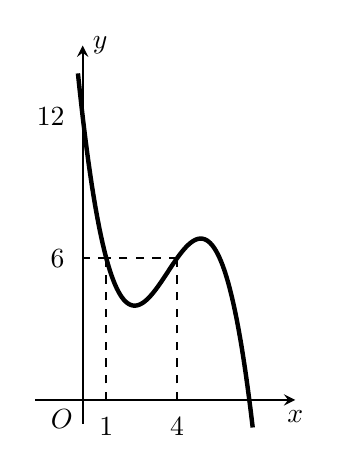
\begin{tikzpicture}[>=stealth, scale=0.3]

    % =================================================================
    % 1. VẼ HỆ TRỤC TỌA ĐỘ Oxy
    % =================================================================
    \draw[->,  thick] (-2.0, 0) -- (9.0, 0) node[below] {$x$};
    \draw[->,  thick] (0, -1.0) -- (0, 15) node[right] {$y$};
    
    % Gốc tọa độ O
    \node[below left] at (0,0) {$O$};

    % =================================================================
    % 2. VẼ ĐƯỜNG CONG ĐỒ THỊ
    % Hợp lý hóa tỷ lệ: Giá trị 12 được thu nhỏ/tịnh tiến để hình vẽ cân đối
    % =================================================================
    \draw[ultra thick, samples=100, domain=-0.2:7.2] 
        plot (\x, {-15/58*\x*\x*\x + 81/29*\x*\x - 495/58*\x +12});
    % =================================================================
    % 3. VẼ CÁC ĐƯỜNG NÉT ĐỨT GIÓNG TỌA ĐỘ
    % =================================================================
    \draw[dashed, thick] (1, 0) -- (1, 6);
    \draw[dashed, thick] (4, 0) -- (4, 6);
    \draw[dashed, thick] (1, 6) -- (0, 6);
    \draw[dashed, thick] (4, 6) -- (1, 6);

    % =================================================================
    % 4. GÁN NHÃN CÁC THÔNG SỐ TRÊN TRỤC
    % =================================================================
    \node[below=3pt] at (1, 0) {$1$};
    \node[below=3pt] at (4, 0) {$4$};
    \node[left=3pt] at (0, 6) {$6$};
    \node[left=3pt] at (0, 12) {$12$};

\end{tikzpicture}
\end{center}

}{
    \textbf{a)} & Hàm số mô phỏng đường trượt là  
    \(y = -\dfrac{15}{58}x^3 + \dfrac{81}{29}x^2 - \dfrac{459}{58}x + 12.\)
    & \textcolor{amberorange}{$\bigcirc$} & \textcolor{amberorange}{$\bigcirc$} \\ \hline
    
    \textbf{b)} & Người chơi trượt đúng theo quỹ đạo đó sẽ được một quãng đường dài 24,47 mét.
    & \textcolor{amberorange}{$\bigcirc$} & \textcolor{amberorange}{$\bigcirc$} \\ \hline
    
    \textbf{c)} & Nếu tốc độ trung bình trên cả đường trượt của người chơi là 2 m/s thì cần 12,37 giây để người đó đến điểm dừng lại.
    & \textcolor{amberorange}{$\bigcirc$} & \textcolor{amberorange}{$\bigcirc$} \\ \hline
    
    \textbf{d)} & Một người chơi mất đúng 6 giây để đến điểm dừng lại, tốc độ trung bình trên cả đường trượt của người chơi đó là 4,12 m/s.
    & \textcolor{amberorange}{$\bigcirc$} & \textcolor{amberorange}{$\bigcirc$} \\
}

% --- CÂU 7 ---
\questionTrueFalse{12}{3}{Mỗi dịp hè về, Bắp được về quê chơi thả diều. Đường bay của nó trong một khoảng thời gian khi gắn hệ trục tọa độ \( Oxy \) được mô phỏng ở hình vẽ. Biết đường bay của nó có dạng đồ thị hàm số bậc ba có điểm cực đại và điểm cực tiểu lần lượt là  
\( A(1;12), \, B\left(4; \frac{78}{11}\right). \)
Đơn vị trên hệ trục tọa độ là mét.

\begin{center}
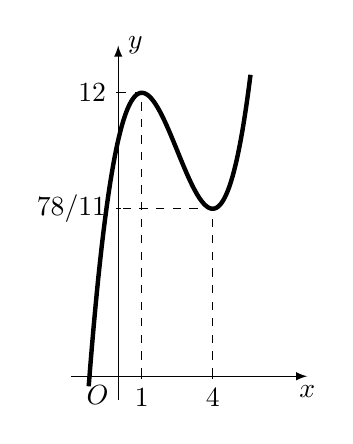
\begin{tikzpicture}[>=latex, scale=0.3]
    % Vẽ hệ trục
    \draw[->] (-2,0) -- (8,0) node[below] {$x$};
    \draw[->] (0,-1) -- (0,14) node[right] {$y$};
    \node[below left] at (0,0) {$O$};
    
    % Đánh dấu các mốc
    \foreach \x in {1,4} {
        \draw (\x,0.1) -- (\x,-0.1) node[below] {$\x$};
    }
    \foreach \y in {78/11,12} {
        \draw (0.1,\y) -- (-0.1,\y) node[left] {$\y$};
    }
    
    % Vẽ đồ thị hàm số bậc 3
    \draw[ultra thick, samples=100, domain=-1.25:5.6] 
        plot (\x, {4/11*\x*\x*\x - 30/11*\x*\x + 48/11*\x + 10});
    \draw[dashed] (1,0) -- (1,12) -- (0,12);
    \draw [dashed] (4,0) --(4,78/11) -- (0,78/11);
   
\end{tikzpicture}
\end{center}

}{
    \textbf{a)} & Hàm số mô phỏng đường bay của con diều trên đoạn \([0;4]\) là       : 
    \(y = \dfrac{4}{11}x^3 - \dfrac{30}{11}x^2 + \dfrac{48}{11}x + 10.\)
    & \textcolor{amberorange}{$\bigcirc$} & \textcolor{amberorange}{$\bigcirc$} \\ \hline
    
    \textbf{b)} & Tại thời điểm con diều ở vị trí cách mặt đất \(Ox\) 7 mét thì nó cách trục \(Oy\) 0,51 mét (kết quả làm tròn đến hàng phần trăm).
    & \textcolor{amberorange}{$\bigcirc$} & \textcolor{amberorange}{$\bigcirc$} \\ \hline
    
    \textbf{c)} & Tại thời điểm con diều ở vị trí cách trục \(Oy\) theo phương ngang 2 mét thì nó cách mặt đất \(Ox\) 17,2 mét (kết quả làm tròn đến hàng phần mười).
    & \textcolor{amberorange}{$\bigcirc$} & \textcolor{amberorange}{$\bigcirc$} \\ \hline
    
    \textbf{d)} & Vị trí ban đầu của con diều cách mặt đất 10 mét.
    & \textcolor{amberorange}{$\bigcirc$} & \textcolor{amberorange}{$\bigcirc$} \\
}

% --- CÂU 8 ---
\questionTrueFalse{12}{4}{Anh Bin có một mảnh vườn hình chữ nhật được chia làm hai khu vực: một khu vực trồng cỏ và một khu vực nuôi bò. Đường cong giới hạn bởi hai khu vực đó khi gắn với hệ trục tọa độ \( Oxy \) được mô phỏng như hình vẽ. Biết đường cong giới hạn đó có dạng là một phần của đồ thị hàm số phân thức
\(y = \dfrac{x^2 + bx + c}{x + n}\)
nhận \( x = 1 \) làm đường tiệm cận đứng. Đơn vị trên hệ trục tọa độ là mét.

\begin{center}
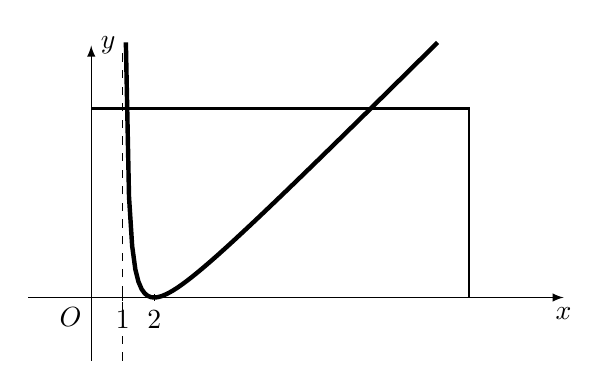
\begin{tikzpicture}[>=latex, scale=0.4]
    % Vẽ hệ trục
    \draw[->] (-2,0) -- (15,0) node[below] {$x$};
    \draw[->] (0,-2) -- (0,8) node[right] {$y$};
    \node[below left] at (0,0) {$O$};
    
    % Đánh dấu các mốc
    \foreach \x in {1,2} {
        \draw (\x,0.1) -- (\x,-0.1) node[below] {$\x$};
    }
    
   \draw[ ultra thick, samples=100, domain=1.1:11] 
        plot (\x, {(\x-2)^2/(\x-1)});
   
    
    % Đường tiệm cận đứng
    \draw[dashed] (1,-2) -- (1,8);
    \draw[thick] (12,0) -- (12,6)--(0,6);

    
\end{tikzpicture}
\end{center}

}{
    \textbf{a)} & Hàm số mô phỏng hình dạng của đường cong giới hạn là \( f(x) = \dfrac{(x-2)^2}{x-1} \).
    & \textcolor{amberorange}{$\bigcirc$} & \textcolor{amberorange}{$\bigcirc$} \\ \hline
    
    \textbf{b)} & Điểm có tọa độ \( (5;9) \) nằm trên đường cong đó.
    & \textcolor{amberorange}{$\bigcirc$} & \textcolor{amberorange}{$\bigcirc$} \\ \hline
    
    \textbf{c)} & Tâm đối xứng của đồ thị hàm số mô phỏng đường cong giới hạn là \( (1;2) \).
    & \textcolor{amberorange}{$\bigcirc$} & \textcolor{amberorange}{$\bigcirc$} \\ \hline
    
    \textbf{d)} & Tại vị trí nằm trên đường cong cách trục \( Oy \) theo phương ngang một đoạn 6 mét thì vị trí đó cách trục hoành một đoạn là 2,3 mét.
    & \textcolor{amberorange}{$\bigcirc$} & \textcolor{amberorange}{$\bigcirc$} \\
}

% --- CÂU 4 ---
\questionTrueFalse{12}{5}{Tại công viên trung tâm, người ta xây một cầu vòm cong bằng thép bắc ngang qua một hồ nước nhỏ. Phần mép cong phía dưới của vòm cầu được thiết kế mô phỏng theo một phần của đồ thị hàm phân thức  
\(y = \dfrac{ax^2 + bx + c}{mx + n} \quad (a \neq 0, m \neq 0)\)
nhận \(x = -1\) là đường tiệm cận đứng. Đơn vị trên hệ trục tọa độ là mét.
\begin{center}
    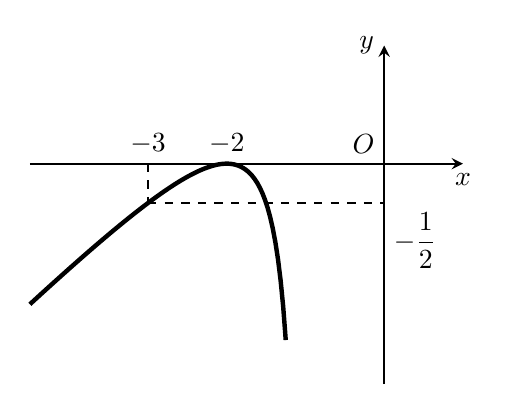
\begin{tikzpicture}[>=stealth, scale=1]

    % =================================================================
    % 1. VẼ HỆ TRỤC TỌA ĐỘ Oxy
    % =================================================================
    \draw[->, thick] (-4.5, 0) -- (1.0, 0) node[below] {$x$};
    \draw[->, thick] (0, -2.8) -- (0, 1.5) node[left] {$y$};
    
    % Gốc tọa độ O
    \node[above left] at (0,0) {$O$};

    % =================================================================
    % 2. VẼ ĐƯỜNG CONG ĐỒ THỊ (HÀM GHÉP ĐỂ ĐẠT ĐỘ DỐC NHƯ HÌNH VẼ)
    % =================================================================
    % Nhánh trái: parabol y = -0.5*(x+2)^2 đi qua (-3, -0.5) và đạt cực đại tại (-2, 0)
    \draw[ultra thick, samples=100, domain=-4.5:-1.25] plot (\x, {(\x*\x + 4*\x +4) /(\x+1)});
    
    

    % =================================================================
    % 3. VẼ CÁC ĐƯỜNG NÉT ĐỨT GIÓNG TỌA ĐỘ
    % =================================================================
    \draw[dashed, thick] (-3, 0) -- (-3, -0.5);
    \draw[dashed, thick] (-3, -0.5) -- (0, -0.5);

    % =================================================================
    % 4. GÁN NHÃN CÁC ĐIỂM TRÊN TRỤC TỌA ĐỘ
    % =================================================================
    \node[above] at (-3, 0) {$-3$};
    \node[above] at (-2, 0) {$-2$};
    \node[below right] at (0, -0.5) {$-\dfrac{1}{2}$};

\end{tikzpicture}
\end{center}
}{
    \textbf{a)} & Hàm số mô phỏng hình dạng vòm cầu là  
    \(f(x) = \dfrac{2(x + 2)^2}{x + 1}.\)
    & \textcolor{amberorange}{$\bigcirc$} & \textcolor{amberorange}{$\bigcirc$} \\ \hline
    
    \textbf{b)} & Điểm có tọa độ \(\left(-5; -\dfrac{9}{4}\right)\) thuộc đồ thị đường cong vòm cầu.
    & \textcolor{amberorange}{$\bigcirc$} & \textcolor{amberorange}{$\bigcirc$} \\ \hline
    
    \textbf{c)} & Đường tiệm cận xiên của đồ thị hàm số mô phỏng hình dạng vòm cầu là \(y = x + 3\).
    & \textcolor{amberorange}{$\bigcirc$} & \textcolor{amberorange}{$\bigcirc$} \\ \hline
    
    \textbf{d)} & Tại vị trí nằm trên vòm cầu cách trục \(Oy\) theo phương ngang một đoạn 4 mét thì điểm đó cách trục hoành một đoạn là \(\dfrac{8}{3}\) mét.
    & \textcolor{amberorange}{$\bigcirc$} & \textcolor{amberorange}{$\bigcirc$} \\
}



% --- CÂU 16 ---
\questionShortAnswer{15}{6}{Một bệnh nhân sau khi trải qua một cuộc phẫu thuật bắt đầu quá trình hồi phục sức khỏe. Sau ngày thứ \( t \) (từ ngày thứ nhất đến ngày thứ 20), bác sĩ đo chỉ số hồi phục tổng quát \( H \) (tính trên thang điểm 200). Kết quả được thống kê lại trong bảng sau:
\begin{table}[h!]
\centering
\renewcommand{\arraystretch}{1.8} % Tăng khoảng cách dòng giúp bảng thông thoáng và đẹp mắt
\begin{tabular}{|c|c|c|c|c|c|}
\hline
$t$ (ngày) & 2 & 5 & 8 & 12 & 16 \\ \hline
\begin{tabular}[c]{@{}c@{}}Chỉ số\\[-3ex] hồi phục H\end{tabular} & 45 & 85 & 115 & 145 & 165 \\ \hline
\end{tabular}
\end{table}

Đồ thị hàm số mô tả quá trình hồi phục của bệnh nhân có dạng  
\(y = \dfrac{at + b}{ct + d} \quad (ad - bc \neq 0, c \neq 0).\) 
Tìm chỉ số hồi phục của bệnh nhân ở ngày thứ 15 (kết quả làm tròn đến hàng đơn vị).}

% --- CÂU 17 ---
\questionShortAnswer{15}{7}{Hai phần đất \( A \) và \( B \) có bề lõm khi gắn hệ trục tọa độ \( Oxy \) được mô phỏng ở hình bên. Biết đường cong trong hình vẽ có dạng đồ thị hàm số bậc ba. Biết rằng đồ thị hàm số có điểm cực đại là \( (2; 18) \) và điểm cực tiểu là \( (-4; 0) \). Đơn vị trên hệ trục tọa độ là mét. Một người đang ở vị trí \( M \) trên phần đất \( A \) đi đến vị trí \( N \) trên phần đất \( B \). Tính khoảng cách \( MN \) (kết quả làm tròn đến hàng phần trăm của mét).

\begin{center}
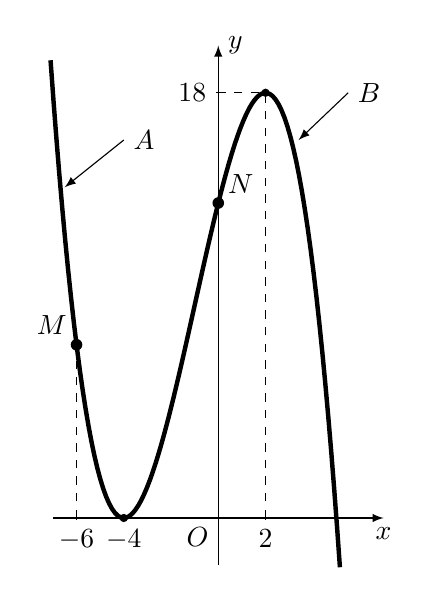
\begin{tikzpicture}[>=latex, scale=0.3]
    % Vẽ hệ trục
    \draw[->] (-7,0) -- (7,0) node[below] {$x$};
    \draw[->] (0,-2) -- (0,20) node[right] {$y$};
    \node[below left] at (0,0) {$O$};
    
    % Đánh dấu các mốc
    \foreach \x in {-6,-4,2} {
        \draw (\x,0.1) -- (\x,-0.1) node[below] {$\x$};
    }
    \foreach \y in {18} {
        \draw (0.1,\y) -- (-0.1,\y) node[left] {$\y$};
    }
    
    % Vẽ đồ thị hàm số bậc 3
    \draw[ultra thick, samples=100, domain=-7.1:5.15] 
        plot (\x, {-1/6*\x*\x*\x - 1/2*\x*\x + 4*\x + 40/3});
    
    % Đánh dấu điểm cực trị
    \fill (2,18) circle (5pt);
    \fill (-4,0) circle (5pt);
    
    % Điểm M và N
    \fill (-6,22/3) circle (7pt) node[above left] {$M$};
    \fill (0,40/3) circle (7pt) node[above right] {$N$};
    \draw[->] (-4,16) node[right] {$A$} -- (-6.5,14);
    \draw[->] (5.5,18) node [right] {$B$} -- (3.4,16);
    \draw[dashed] (2,0) -- (2,18) -- (0,18);
    \draw [dashed] (-6,0) -- (-6,20/3);
\end{tikzpicture}
\end{center}}

% --- CÂU 18 ---
\questionShortAnswer{15}{8}{Bạn Lan đang ôn luyện từ vựng để chuẩn bị cho kì thi. Sau tuần thứ \( t \) (từ tuần thứ 2 đến tuần thứ 15), giáo viên ghi lại tổng số từ vựng mà Lan đã học được. Bảng sau thể hiện số liệu mà giáo viên đã thống kê lại:

\begin{table}[h!]
\centering
\renewcommand{\arraystretch}{1.8} % Giữ khoảng cách dòng rộng rãi, thông thoáng giống ảnh mẫu
\begin{tabular}{|c|c|c|c|}
\hline
$t$ (tuần) & 2 & 4 & 10 \\ \hline
Số từ đã học & 60 & 120 & 165 \\ \hline
\end{tabular}
\end{table}

Biết rằng hàm số mô tả tổng số từ vựng mà Lan đã học được có dạng \( y = \dfrac{at + b}{ct + d} \) (\( ad - bc \neq 0, c \neq 0 \)). Đồ thị hàm số mô tả tổng số từ vựng có tổng hoành độ và tung độ của tâm đối xứng là bao nhiêu (kết quả làm tròn đến hàng đơn vị)?}

% --- CÂU 19 ---
\questionShortAnswer{15}{9}{Bạn Hoàng treo một sợi dây trang trí thành hình dạng một đường cong có đồ thị là hàm số bậc ba khi gắn hệ trục tọa độ Oxy được mô phỏng ở hình vẽ. Đơn vị trên hệ trục là centimet. Biết rằng độ dài đường cong có phương trình \( y = f(x) \) từ điểm \( A(a; f(a)) \) tới điểm \( B(b; f(b)) \) với \( a < b \) được tính bởi công thức  
\(T = \int_a^b \sqrt{1 + (f'(x))^2} \, dx.\)
Tính độ dài của sợi dây đó (đơn vị: centimet, làm tròn kết quả đến hàng phần mười).

\begin{center}
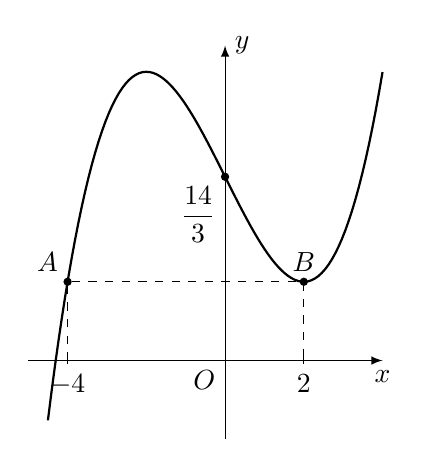
\begin{tikzpicture}[>=latex, scale=0.5]
    % Vẽ hệ trục
    \draw[->] (-5,0) -- (4,0) node[below] {$x$};
    \draw[->] (0,-2) -- (0,8) node[right] {$y$};
    \node[below left] at (0,0) {$O$};
    
    % Đánh dấu các mốc
    \foreach \x in {-4,2} {
        \draw (\x,0.1) -- (\x,-0.1) node[below] {$\x$};
    }
    
    % Vẽ đồ thị hàm số bậc 3
    \draw[thick, samples=100, domain=-4.5:4] 
        plot (\x, {1/6*\x^3 - 2*\x + 14/3});
    
    % Điểm A và B
    \fill (0,14/3) circle (3pt) node[below left] {$\dfrac{14}{3}$};
    \fill (-4,2) circle (3pt) node[above left] {$A$};
    \fill (2,2) circle (3pt) node[above] {$B$};
    \draw[dashed] (-4,0) -- (-4,2) -- (2,2) -- (2,0);
\end{tikzpicture}
\end{center}}

% --- CÂU 20 ---
\questionShortAnswer{15}{10}{Bắp và các bạn được vào chơi tại một mảnh đất hình chữ nhật được chia làm hai khu vực: một khu vực an toàn và một khu vực nguy hiểm. Đường cong giới hạn bởi hai khu vực đó khi gắn với hệ trục tọa độ Oxy được mô phỏng như hình vẽ. Biết đường cong giới hạn đó có dạng là một phần của đồ thị hàm số phân thức \( y = \dfrac{x^2 + bx + c}{x + n} \) nhận \( x = 2 \) làm đường tiệm cận đứng. Đơn vị trên hệ trục tọa độ là mét. Tại vị trí nằm trên đường cong cách trục Oy theo phương ngang một đoạn 4,5 mét thì vị trí đó cách trục hoành một đoạn là bao nhiêu centimet (kết quả làm tròn đến hàng phần mười)?

\begin{center}
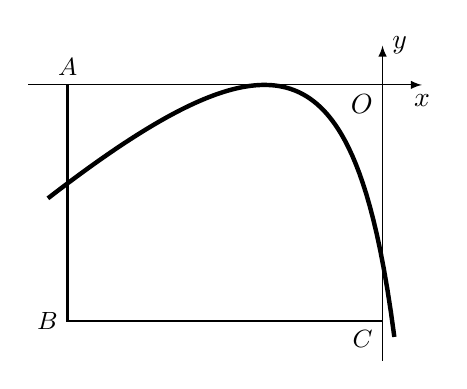
\begin{tikzpicture}[>=latex, scale=0.5]
    % Vẽ hệ trục
    \draw[->] (-9,0) -- (1,0) node[below] {$x$};
    \draw[->] (0,-7) -- (0,1) node[right] {$y$};
    \node[below left] at (0,0) {$O$};
    
    % Vẽ đồ thị hàm số
    \draw[ultra thick, samples=100, domain=-8.5:0.3] 
        plot (\x, {(\x + 3)^2/(\x - 2)});
    \draw [thick] (-8,0) -- (-8,-6) -- (0,-6);
    \node [above] at (-8,0) {\small$A$};
    \node [left] at (-8,-6) {\small $B$};
    \node [below left] at (0,-6) {\small $C$};

\end{tikzpicture}
\end{center}}

% --- CÂU 21 ---
\questionShortAnswer{15}{11}{Một học sinh đang luyện nghe Tiếng Anh để chuẩn bị thi định kì. Sau tuần thứ \( t \) (tính từ tuần thứ 1 đến tuần thứ 12), bạn ấy đã thống kê lại được tổng số giờ luyện nghe đã tích lũy được trong bảng số liệu sau:  

\begin{table}[h!]
\centering
\renewcommand{\arraystretch}{2.0} % Tăng khoảng cách dòng để các phân số không bị chạm vào đường kẻ
\begin{tabular}{|c|c|c|c|c|}
\hline
$t$ (tuần) & 1 & 3 & 6 & 10 \\ \hline
Số giờ nghe & $\dfrac{23}{2}$ & 23 & $\dfrac{92}{3}$ & $\dfrac{460}{13}$ \\ \hline
\end{tabular}
\end{table}

Biết rằng hàm số mô tả tổng số giờ luyện nghe của bạn học sinh đó có dạng  
\(y = \dfrac{at + b}{ct + d} \quad (ad - bc \neq 0, c \neq 0).\) 
Đến tuần thứ 12, tổng số giờ luyện nghe của bạn ấy đạt được là bao nhiêu?}

% --- CÂU 22 ---
\questionShortAnswer{15}{12}{Trong hệ trục tọa độ \( Oxy \), cho đồ thị hàm số  
\((C): y = \dfrac{x^2 + x + 1}{x + 1}; \, x > -1\) 
mô tả chuyển động của một chiếc thuyền trên biển, một trạm phát sóng đặt tại điểm \( I(-1; -1) \). Biết hoành độ điểm \( M \) thuộc đồ thị \( (C) \) mà tại đó thuyền thu được sóng tốt nhất là  
\(x_0 = \dfrac{1}{\sqrt{a}} - b\)  
(loại trừ các điều kiện ảnh hưởng đến việc thu phát sóng). Tính \( a + b \).}

% --- CÂU 23 ---
\questionShortAnswer{15}{13}{Bạn Nam phóng một chiếc máy bay giấy cỡ nhỏ trong không trung. Đường bay của nó khi gắn hệ trục tọa độ Oxy được mô phỏng ở hình vẽ. Biết đường bay của nó có dạng đồ thị hàm số bậc ba (xem hình vẽ); vị trí máy bay bắt đầu di chuyển cách điểm máy bay rơi tại gốc tọa độ theo phương ngang là 1,5 mét. Điểm tiếp đất của máy bay là điểm cực tiểu của đồ thị hàm số. Trước đó, độ cao cực đại mà máy bay đạt được ứng với điểm có tọa độ \( (0; 4) \). Đơn vị trên hệ trục tọa độ là mét. Tính khoảng cách giữa vị trí ban đầu và vị trí rơi của máy bay (đơn vị: mét, kết quả làm tròn đến hàng phần trăm).

\begin{center}
\begin{tikzpicture}[>=latex, scale=0.8]
    % =================================================================
    % 1. VẼ MÁY BAY GIẤY BẰNG VECTOR TIKZ (Phía bên trái đồ thị)
    % =================================================================
    \begin{scope}[shift={(-2.3, 1.5)}, scale=0.2, rotate=15]
        % Thân dưới máy bay giấy
        \draw[thick, fill=white] (0,0) -- (2,-0.8) -- (0.5,-1.2) -- cycle;
        % Cánh lớn phía trước
        \draw[thick, fill=white] (0,0) -- (4,0.8) -- (2,-0.8) -- cycle;
        % Cánh gập phía sau
        \draw[thick, fill=white] (0,0) -- (4,0.8) -- (0.8,0.5) -- cycle;
        % Nếp gấp nhỏ bên trong cánh
        \draw[thick] (0.8,0.5) -- (2,-0.8);
    \end{scope}
    % Vẽ hệ trục
    \draw[->] (-2.5,0) -- (5,0) node[below] {$x$};
    \draw[->] (0,-1) -- (0,5.5) node[right] {$y$};
    \node[below left] at (0,0) {$O$};
    
    % Đánh dấu các mốc
   
    \draw (0.1,4) -- (-0.1,4) node[left] {$4$};
    
    % Vẽ đồ thị hàm số bậc 3
    \draw[thick, samples=100, domain=-1.5:4] 
       plot (\x, {1/8*\x*\x*\x - 3/4*\x*\x + 4});
    
    % Đánh dấu điểm cực đại và cực tiểu
    \fill (0,4) circle (3pt);
    \fill (4,0) circle (3pt) node [below] {$4$};
    \draw[dashed] (-1.5,0) -- (-1.5,2);
    % Vị trí ban đầu
    \fill (-1.5,0) circle (3pt) node[below] {$1,5$};
\end{tikzpicture}
\end{center}}

% --- CÂU 24 ---
\questionShortAnswer{15}{14}{Một phần của đường chạy của tàu lượn siêu tốc khi gắn hệ trục tọa độ Oxy được mô phỏng ở hình vẽ. Biết đường chạy của nó có dạng đồ thị hàm số bậc ba. Biết đồ thị hàm số đi qua các điểm \((-1; 6)\), \((0; 5)\) và nhận \((3; 3)\) làm điểm cực tiểu. Nếu một người tham gia chơi trò tàu lượn siêu tốc, tại thời điểm \(t_1\), người đó ở vị trí có hoành độ là \(-3\), tại thời điểm \(t_2\) (\(t_2 > t_1\)), người đó ở vị trí có tung độ là 4,4. Tính khoảng cách giữa hai vị trí đó theo đơn vị mét (kết quả làm tròn đến hàng phần trăm, đơn vị trên hệ trục tọa độ là mét).

\begin{center}
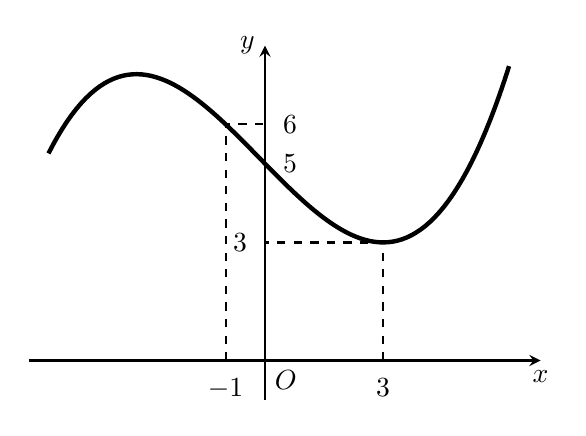
\begin{tikzpicture}[>=stealth, scale=0.5]

    % =================================================================
    % 1. VẼ HỆ TRỤC TỌA ĐỘ Oxy
    % =================================================================
    \draw[->, thick] (-6.0, 0) -- (7.0, 0) node[below] {$x$};
    \draw[->, thick] (0, -1.0) -- (0, 8.0) node[left] {$y$};
    
    % Gốc tọa độ O
    \node[below right] at (0,0) {$O$};

        \draw[ultra thick, samples=100, domain=-5.5:6.2] 
        plot (\x, {5/144*\x*\x*\x + 1/72*\x*\x - 49/48*\x + 5});

    % =================================================================
    % 3. VẼ CÁC ĐƯỜNG NÉT ĐỨT GIÓNG TỌA ĐỘ
    % =================================================================
    % Gióng điểm tại x = -1 (y = 3.4)
    \draw[dashed, thick] (-1, 0) -- (-1, 6) -- (0, 6);
    
    % Gióng điểm cực tiểu tại x = 3 (y = 1.2)
    \draw[dashed, thick] (3, 0) -- (3, 3) -- (0, 3);

    % =================================================================
    % 4. GÁN NHÃN CÁC GIÁ TRỊ TRÊN TRỤC
    % =================================================================
    % Trục hoành (Ox)
    \node[below=3pt] at (-1, 0) {$-1$};
    \node[below=3pt] at (3, 0) {$3$};
    
    % Trục tung (Oy)
    \node[right=3pt] at (0, 6) {$6$};
    \node[right=3pt] at (0, 5) {$5$}; % Giao điểm đồ thị với Oy
    \node[left=3pt] at (0, 3) {$3$};

\end{tikzpicture}
\end{center}}

% --- CÂU 25 ---
\questionShortAnswer{15}{15}{Mít được về quê chơi thả diều. Đường bay của nó trong một khoảng thời gian khi gắn hệ trục tọa độ Oxy được mô phỏng ở hình vẽ. Biết đường bay của nó có dạng đồ thị hàm số bậc ba có điểm cực đại và điểm cực tiểu lần lượt là \( A(-1;8) \), \( B(0;6) \). Đơn vị trên hệ trục tọa độ là mét. Biết vị trí ban đầu của diều cách trục Oy theo phương ngang một khoảng 1,5 mét, tìm độ cao của diều lúc đó theo đơn vị mét.

\begin{center}
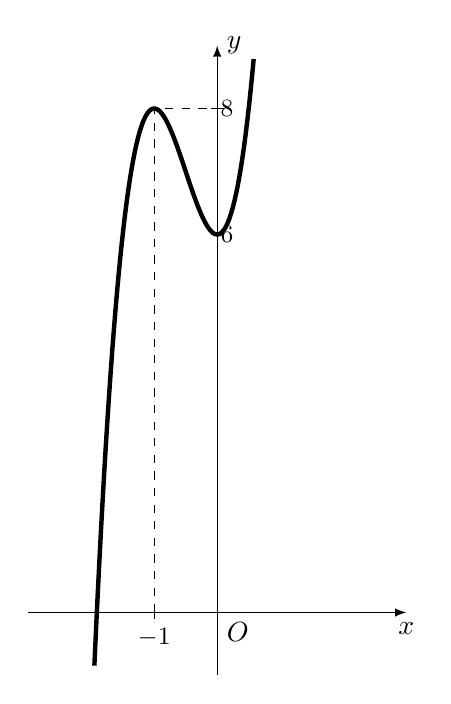
\begin{tikzpicture}[>=latex, scale=0.8]
    % Vẽ hệ trục
    \draw[->] (-3,0) -- (3,0) node[below] {$x$};
    \draw[->] (0,-1) -- (0,9) node[right] {$y$};
    \node[below right] at (0,0) {$O$};
    
    % Đánh dấu các mốc
    \foreach \x in {-1} {
        \draw (\x,0.1) -- (\x,-0.1) node[below] {\small$\x$};
    }
    \foreach \y in {6,8} {
        \draw (0.1,\y) -- (-0.1,\y) node[right] {\small$\y$};
    }
    
    % Vẽ đồ thị hàm số bậc 3
    \draw[ultra thick, samples=100, domain=-1.95:0.58] 
       plot (\x, {4*\x*\x*\x + 6*\x*\x + 6});
    \draw[dashed] (-1,0) -- (-1,8) -- (0,8);
\end{tikzpicture}
\end{center}}

% --- CÂU 26 ---
\questionShortAnswer{15}{16}{Chị Dung có một mảnh đất hình vuông có cạnh là 9 mét. Chị ấy quyết định chia miếng đất thành ba phần. Phần ở giữa chị ấy nuôi gà. Hai phần ở góc chị ấy dự tính dùng để trồng các loại rau. Để ngăn gà không sang được phần trồng rau, chị ấy làm các hàng rào gỗ có hình dạng là đường cong của đồ thị hàm số  
\[y = \frac{ax + b}{cx + d} \quad (ad - bc \neq 0; c \neq 0).\]
Khi đó gắn hệ trục tọa độ Oxy như hình vẽ. Biết rằng đồ thị hàm số nhận \(x = 2; y = -1\) làm các đường tiệm cận. Đơn vị trên hệ trục là mét. Khoảng cách ngắn nhất giữa hai vị trí nằm trên hai hàng rào là bao nhiêu mét (kết quả làm tròn đến hàng phần mười)?

\begin{center}
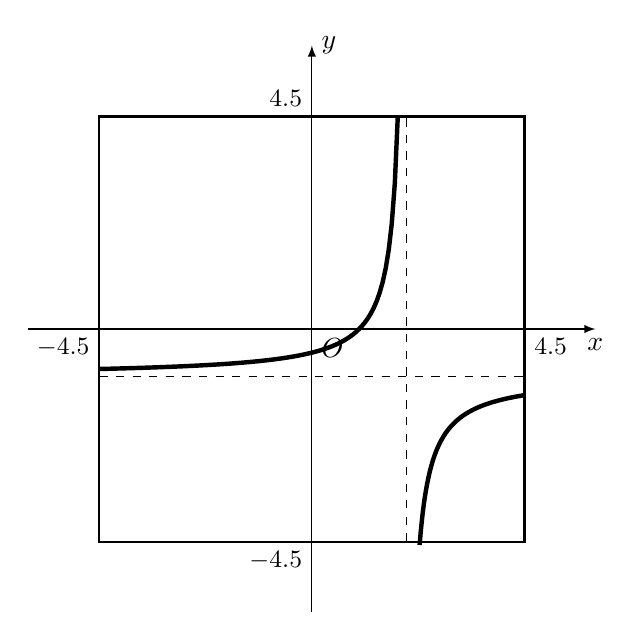
\begin{tikzpicture}[>=latex, scale=0.6]
    % Vẽ hình vuông
    \draw[thick] (-4.5,-4.5) rectangle (4.5,4.5);
    % Vẽ hệ trục
    \draw[->] (-6,0) -- (6,0) node[below] {$x$};
    \draw[->] (0,-6) -- (0,6) node[right] {$y$};
    \node[below right] at (0,0) {$O$};
    % Vẽ đường cong
    \draw[ultra thick, samples=100, domain=2.28:4.5] 
        plot (\x, {(-\x+1)/(\x-2)});
    \draw[ultra thick, samples=100, domain=-4.5:1.82] 
        plot (\x, {(-\x+1)/(\x-2)});
    
    % Đường tiệm cận
    \draw[dashed] (2,-4.5) -- (2,4.5) ;
    \draw[dashed] (-4.5,-1) -- (4.5,-1) ;
    \node [below left] at (-4.5,0) {\small $-4.5$};
    \node [below right] at (4.5,0) {\small $4.5$};
    \node [above left] at (0,4.5) {\small $4.5$};
    \node [below left] at (0,-4.5) {\small $-4.5$};
\end{tikzpicture}
\end{center}}


\end{document}
